% ============================================================
% 4. EXPERIMENTS
% ============================================================
% DRAFT v0.1 (2026-08-13). Solid draft, NOT final. Seams marked with \flag
% or "FLAG:". All numbers staged/confirmed on the Notion working page unless
% FLAGged. Erfan's horizon subsection is a labelled stub, not prose.
% ============================================================
\section{Experiments}
\contrib{lead: Parsa (controls/results); Erfan (horizon table, \S\ref{subsec:horizon})}

This section works through one question: does conditioning a frozen V-JEPA~2
predictor on egocentric gaze and hand improve short-horizon action anticipation,
and if not, why? We fix the protocol (\S\ref{subsec:protocol}), build the
controls that separate a token-count confound from a real content effect
(\S\ref{subsec:controls}), and then report the null and the five diagnostics that
characterise it (\S\ref{subsec:diagnostics}). A companion set of
experiments then varies the training rather than the input
(\S\ref{subsec:training-ablation}). Together they license the design-stage
decision of \S\ref{subsec:b4}. The one residual effect and its
limits follow (\S\ref{subsec:dissociation}), then the sample-size mechanism that
binds the picture together (\S\ref{subsec:ddn}). A closing horizon analysis
(\S\ref{subsec:horizon}) characterises how far ahead the behavioral signal is
legible in the frozen representation at all.

\paragraph{Three venues, and which one carries which claim.}
The work spans three evaluation venues that answer different questions, and
keeping them apart is essential to reading the results correctly. The EK100 result
(\S\ref{subsec:controls}) is \emph{signal-absent}: EK100 provides no gaze or hand
at evaluation, so the behavioral slots are masked, and a null there tells us
whether a behaviorally-trained predictor transfers downstream, nothing more. The
diagnostics, the dissociation, and the sample-size analysis
(\S\ref{subsec:diagnostics}--\ref{subsec:ddn}) all live in the \emph{signal-present}
venue, a direct probe on HD-EPIC~P01, which is the only setting that can test the
gaze/hand-to-motion mechanism directly. The third venue is the conditioning objective itself
(\S\ref{subsec:training-ablation}, \S\ref{subsec:horizon}): feature-space
prediction error, trained on HD-EPIC~P01--P07 and evaluated on held-out
participants. It is the only venue here that is cross-participant, and it is
where the ablations that vary training rather than input are run. The decision to
retire the stronger pathway (\S\ref{subsec:b4}) rests on the signal-present
diagnostics and on those ablations; the EK100 null is corroborating context, not
the basis for it. We do not read a
signal-absent null as evidence about the signal's content.

% ------------------------------------------------------------
\subsection{Data and protocol}
\label{subsec:protocol}

The ViT-L feasibility fine-tuning below is trained on
HD-EPIC~\citep{perrett2025hdepic} P01 (the ViT-G checkpoint carrying every
anticipation result was trained on P01--P07 and validated on P08;
\S\ref{subsec:method-setup}),
whose Aria-quality annotations supply per-frame three-dimensional gaze
(yaw, pitch, depth) and a twelve-dimensional two-hand pose signal. The
anticipation probe is evaluated on the EPIC-KITCHENS-100 (EK100)
action-anticipation task~\citep{damen2022ek100}, which asks a model to predict
the verb, noun, and verb--noun action of a segment from a context clip ending a
fixed interval before onset; performance is reported as mean-class recall@5.

\paragraph{A single-participant evaluation scope.}
We state at the outset a framing constraint that governs the interpretation of
every result below. Although the EK100 validation annotations for participants
P01--P05 comprise \num{2213} clips, the evaluation in practice ran on P01 alone:
of the P01--P05 videos, only the thirteen P01 videos were present on disk at run
time, and the loader's missing-file filter silently drops the
remainder.\footnote{The dataloader emits a \texttt{file path not found} line per
absent video; every Phase-5/6 log contains 620 such lines, leaving
\texttt{P01\_102}--\texttt{P01\_109} (train) and \texttt{P01\_11}--\texttt{P01\_15}
(val). The resulting clip counts, \num{2401} train and \num{870} val, are
confirmed three independent ways by the dataloader iteration counts across
seeds.} The evaluated set is therefore \textbf{\num{870} validation and
\num{2401} training clips, P01 only}; the ``P01--P05 (\num{2213})'' figure
describes the annotation subset, not the data actually seen. This is not a
cosmetic correction. It makes the conditioning null a single-participant result,
accounts directly for the small between-seed spread reported below, and is the
mechanism to which we return in \S\ref{subsec:ddn} and in the limitations.

\paragraph{Compute.}
The work ran across two clusters. The earlier conditioning experiments, including
the confounded pilot of \S\ref{subsec:bg-origin}, were carried out on a single
NVIDIA L40S GPU ($\approx$46\,GB) under a \texttt{tcsh} environment. The project
data and checkpoints were then transferred to a second cluster, on which the
frozen-probe training and evaluation reported in this paper were run.\footnote{The
second cluster's GPU and CPU specifications are not recorded in the sources
available to us at writing, and we report the environment only for completeness.} All reported anticipation numbers come from the second cluster; no
result in this paper depends on the compute environment, and the binding
constraint on the results is sample size rather than compute
(\S\ref{subsec:ddn}).

\paragraph{Feasibility of the conditioning target.}
Before probing anticipation, we confirm the behavioral predictor was trainable
at all. Fine-tuning the V-JEPA~2 predictor on HD-EPIC~P01 (ViT-L, 20 epochs)
reduces the per-epoch mean smooth-$L_1$ prediction loss from
$1.207$ to $1.019$, with the curve essentially flat after roughly the fifth
epoch (epoch~5 mean $1.063$; epoch~15 mean $1.034$).\footnote{The same run's
raw first- and last-iteration values are $2.135$ and $1.002$; these are a
different unit from the per-epoch means and are not mixed with them.} The signal
is learnable, then, but its marginal return saturates early. That is an honest
feasibility ceiling, not a training failure.

\begin{figure}[t]
  \centering
  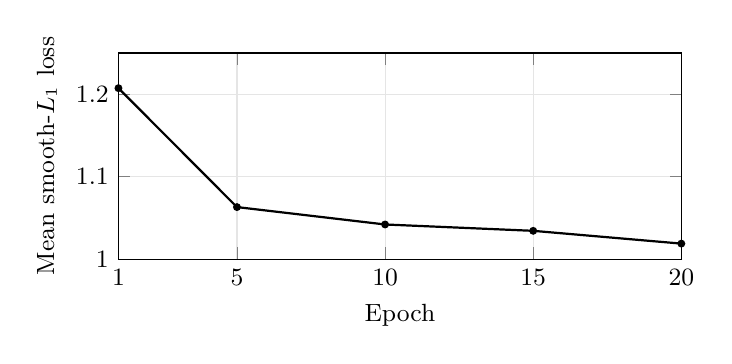
\begin{tikzpicture}
    \begin{axis}[
      width=0.72\linewidth, height=4.2cm,
      xlabel={Epoch}, ylabel={Mean smooth-$L_1$ loss},
      xmin=1, xmax=20, ymin=1.0, ymax=1.25,
      xtick={1,5,10,15,20},
      tick label style={font=\small}, label style={font=\small},
      grid=major, grid style={gray!20},
    ]
      \addplot[thick, mark=*, mark size=1pt] coordinates {
        (1,1.2074) (5,1.0632) (10,1.0421) (15,1.0344) (20,1.0189)
      };
    \end{axis}
  \end{tikzpicture}
  \caption{Per-epoch mean prediction loss for the behavioral predictor
  (HD-EPIC~P01, ViT-L, 20 epochs). The loss falls from $1.207$ to $1.019$ but is
  essentially flat after epoch~5, indicating an early feasibility ceiling rather
  than a training failure. Intermediate points ($1.063$, $1.042$, $1.034$) are
  the epoch~5/10/15 means. The curve is drawn from the five recorded checkpoints.}
  \label{fig:loss}
\end{figure}

% ------------------------------------------------------------
\subsection{Controls: separating token count from content}
\label{subsec:controls}

A conditioned run differs from an unconditioned one in more than the presence of
the behavioral signal. To expose anticipatory content, the probe is fed not only
the encoder's \num{1568} output tokens ($T\cdot N = 8\times196$) but also the
predictor's last predicted-frame block appended alongside them, taking the probe
input to \num{1764} tokens ($(T{+}1)\cdot N = 9\times196$). A naive
conditioned-versus-unconditioned comparison therefore confounds any content
effect with the effect of simply giving the probe more tokens. We break the
confound with a control family that holds the target constant and varies only
what fills the appended block:
\begin{itemize}
  \item \textbf{6a, encoder only} (\num{1568} tokens): no appended block.
  \item \textbf{6b, zero padding} (\num{1764} tokens): the appended block is zeros.
  \item \textbf{6c, content-free repeat} (\num{1764} tokens): the appended block
        repeats an existing frame, matching the token count without adding
        information.
  \item \textbf{Behavioral} (\num{1764} tokens): the appended block is the real
        prediction from the behaviorally-conditioned predictor.
\end{itemize}
The attentive pooler used for readout carries no positional encoding in its
attention path at any probed depth, so it is permutation-invariant over the token
axis, which is what makes 6b and 6c valid token-count-matched controls. We show
the controls before the headline comparison because the null only means something
once the token-count effect has been subtracted out.

The comparison is in Table~\ref{tab:main}, and the headline reading is best-epoch,
where the behavioral arm does not separate from its token-count-matched controls:
the behavioral-minus-6a gap is $-0.013$\,pp. Whatever advantage conditioning
appears to give is a token-count effect, not a content effect. The final-epoch
column tells a superficially different story that we address directly below, so
that it is not misread.

\begin{table}[t]
  \caption{Control family for the input-conditioning null (EK100 action R@5,
  \%, P01, signal-absent). Best-epoch values headline, with final-epoch
  (epoch~10) in parentheses. Best-epoch is the honest comparison, though it is
  selected on the reported validation set: the behavioral arm does not separate
  from its token-count-matched controls (behavioral $-$ 6a $= -0.013$\,pp). On
  final-epoch the behavioral arm leads by $0.15$--$0.27$\,pp, but only because it
  is the one arm that does not decay after epoch~8; that is a decay asymmetry, not
  a sign of the signal. The 6b and 6c conditions were run at two seeds, the third
  having been dropped once the direction was closed.}
  \label{tab:main}
  \centering
  \begin{tabular}{lccccc}
    \toprule
    Condition & Tokens & Seed 42 & Seed 43 & Seed 44 & Mean \\
    \midrule
    6a encoder only        & 1568 & 3.69 (3.38) & 3.44 (3.16) & 3.72 (3.54) & 3.62 (3.36) \\
    6b zero padding        & 1764 & 3.61 (3.61) & 3.59 (3.22) & ---         & 3.60 (3.42) \\
    6c content-free repeat & 1764 & 3.77 (3.46) & 3.31 (3.13) & ---         & 3.54 (3.29) \\
    Behavioral             & 1764 & 3.58 (3.48) & 3.49 (3.47) & 3.75 (3.75) & 3.61 (3.57) \\
    \bottomrule
  \end{tabular}
\end{table}

% ------------------------------------------------------------
\subsection{Five diagnostics on the frozen predictor}
\label{subsec:diagnostics}

Two readings of the null remained open after the controls: either the injection
pathway is too weak to expose whatever the signal carries, or the signal does
not carry action-relevant information at this horizon. The first recommends a
stronger architecture; the second recommends abandoning input-level conditioning
altogether. Rather than build a stronger pathway on the assumption that it would
help, we ran five diagnostics against the frozen predictor and the behavioral
signal directly (Table~\ref{tab:diagnostics}). They converge.

\begin{table}[t]
  \caption{Diagnostics bearing on whether a stronger pathway could recover
  anticipatory information. Full outputs in Appendix~\ref{sec:extended}.}
  \label{tab:diagnostics}
  \centering
  \small
  \begin{tabular}{lll}
    \toprule
    Diagnostic & Measurement & Interpretation \\
    \midrule
    Output shift (real vs.\ masked)      & relative $L_2 = 9.9\%$
      & the signal reaches the output \\
    Average-error gap (PEVA-1)           & $0.055\%$; real$>$masked 172/220, $p\approx3\times10^{-19}$
      & detectable but negligible \\
    Discrimination (PEVA-2)              & top-1 gap $0.0000$; 0/220 discordant
      & no discriminative margin \\
    Attention on the slot (Test A)       & $28.6\times$ (gaze) / $35.4\times$ (hand) uniform
      & the slot is heavily attended\dots \\
    Attention change, real vs.\ masked   & $\le 0.1\%$, negative in sign
      & \dots but indifferent to content \\
    Signal-alone anticipation (Test B)   & $12.2\%$ vs.\ $10.4\%$ prior ($+1.8$\,pp)
      & faint at source \\
    \bottomrule
  \end{tabular}
\end{table}

The attention result is the pivotal one. The predictor attends to the gaze and
hand slots at roughly twenty-nine to thirty-five times the uniform rate, so the
signal is clearly not being ignored on positional grounds. But replacing the real
signal with the mask token barely moves the attention; if anything the mask draws
marginally more. The model attends to where the signal sits and stays indifferent to what it says.
\S\ref{subsec:training-ablation} shows that this routing is
inherited from the action-conditioned pretraining rather than learned here, which
makes the absence of headroom a property of the architecture rather than of this
particular run. Key-biasing, the first mechanism a stronger, GazeQwen-style
pathway~\citep{pham2026gazeqwen} would add, needs headroom in exactly this
attention magnitude, and there is none to work with. Put beside the direct probe,
where the signal beats a class prior by only $1.8$ points, the reading is
consistent: the signal is registered but faint, and no rearrangement of the
pathway can recover information that a direct probe can barely find.

\begin{figure}[t]
  \centering
  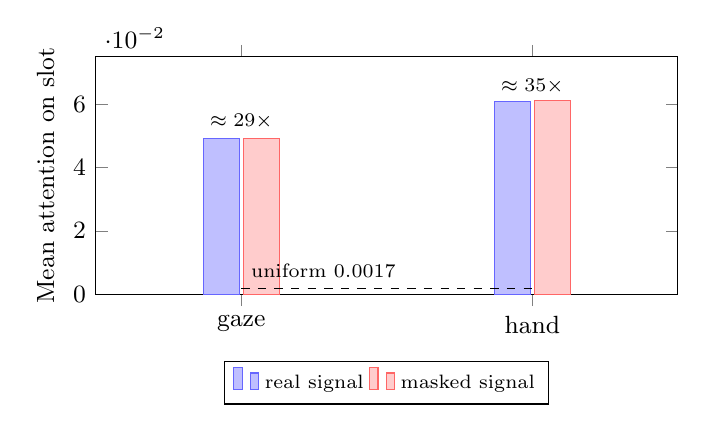
\begin{tikzpicture}
    \begin{axis}[
      width=0.74\linewidth, height=4.6cm,
      ybar=1.5pt, bar width=13pt,
      symbolic x coords={gaze, hand},
      xtick=data,
      ymin=0, ymax=0.075,
      ytick={0,0.02,0.04,0.06},
      ylabel={Mean attention on slot},
      enlarge x limits=0.5,
      tick label style={font=\small}, label style={font=\small},
      legend style={font=\scriptsize, at={(0.5,-0.28)}, anchor=north, legend columns=-1},
    ]
      \addplot[draw=blue!60, fill=blue!25] coordinates {(gaze,0.049080) (hand,0.060709)};
      \addplot[draw=red!60, fill=red!20]  coordinates {(gaze,0.049155) (hand,0.061035)};
      % uniform baseline, labelled
      \addplot[black, dashed, sharp plot, update limits=false]
        coordinates {(gaze,0.001716) (hand,0.001716)};
      \node[font=\scriptsize, anchor=south west] at (axis cs:gaze,0.0022) {uniform $0.0017$};
      % multiples above each pair
      \node[font=\scriptsize] at (axis cs:gaze,0.0545) {$\approx 29\times$};
      \node[font=\scriptsize] at (axis cs:hand,0.0655) {$\approx 35\times$};
      \legend{real signal, masked signal}
    \end{axis}
  \end{tikzpicture}
  \caption{Attention on the behavioral slots, real versus masked signal, against
  the uniform baseline (dashed, $0.0017$). Both slots draw roughly $29$--$35\times$
  uniform attention, yet the real and masked bars are indistinguishable
  (gaze $0.0491$ vs.\ $0.0492$; hand $0.0607$ vs.\ $0.0610$): the predictor
  attends to where the signal sits, not to what it says.}
  \label{fig:attention}
\end{figure}

% ------------------------------------------------------------
\subsection{Varying the training instead of the input}
\label{subsec:training-ablation}
\contrib{lead: Erfan}

Every diagnostic in \S\ref{subsec:diagnostics} holds one predictor fixed and
varies what is fed to it. That instrument can establish whether the model
responds to the signal, but it cannot separate the value of the information from
the cost of withholding an input the model was organised around: both appear as
the same difference. Separating them requires varying the \emph{training}. The
experiments below do exactly that, and they do it on the same warm-start
checkpoint that carries every anticipation result above
(\S\ref{subsec:method-setup}): its training run is re-executed with the
behavioral signal ablated, and the two models are compared directly. They are
scored on the conditioning objective, feature-space prediction error over
held-out participant~P08, on a fixed set of \num{96} clips, paired throughout.

\paragraph{The pathway is alive, graded, and small.}
Holding the video fixed and perturbing the gaze input by a known angle gives a
response that is monotone and near-linear from $1^\circ$ to $10^\circ$
($0.0012 \rightarrow 0.0024 \rightarrow 0.0061 \rightarrow 0.0130$, a factor of
eleven in output movement for a factor of ten in angle) and super-linear beyond,
reaching $0.081$ at $45^\circ$, about $14\%$ of the movement caused by
replacing the entire visual context. An identity control, the same forward pass
run twice, is exactly zero on all \num{96} clips, so every non-zero figure above
is signal rather than nondeterminism. The first reading of the null, that the
signal never reaches the predictor or that the pathway failed to train, is
therefore false. The channel functions; its gain is simply small.

\paragraph{Attention, quantified.}
On a $258$-token sequence the uniform share of a visual token's attention falling
on the gaze token is $1/258 = 0.388\%$. Measured, visual tokens spend
$12$--$26\%$ of their attention there, and in one head the gaze token takes
essentially the entire attention mass, $258\times$ uniform. The same
measurement on the \emph{untrained} model (action-conditioned weights, randomly
initialised projectors, no fine-tuning) already gives roughly $38\times$
uniform, and three epochs of training move it only to about $42\times$. The
routing is inherited from the action-conditioned pretraining that placed robot
action and state tokens in that position; training barely touches it.

\paragraph{Training built the pathway up, not down.}
A natural explanation for a null is that optimisation suppressed the new channel.
It did the opposite: the gaze projector's weight norm \emph{grew} $15.7\%$ against
its initialisation while every other trained parameter under the same weight decay
stayed within $0.05\%$ of its own.\footnote{The mask-token baseline used
throughout is itself a choice worth bounding. On the same checkpoint and clips the
conditioning gap is $+0.0007$ against mean imputation, $+0.0011$ against the mask
token and $+0.0022$ against zeros, a spread of $0.0015$ that is wider than the
smallest of the three effects.}

\paragraph{Most of what the projector learned is a constant.}
The mechanism behind the null is visible in the projector's parameters. Its bias
moved from exactly $0.000$ to $0.572$ against a weight norm of $1.270$, so a large
share of what it learned does not depend on gaze at all. That accounts for the pattern the
input-side diagnostics see: masking gaze moves the
prediction $5.2\times$ further than replacing it with a \emph{different} clip's
gaze ($0.084$ versus $0.016$). The model separates ``some gaze'' from ``no gaze''
far more sharply than one gaze from another, which is how heavy attention
coexists with small sensitivity: the heavily attended token is mostly a constant.\footnote{Shuffling gaze across time within a clip, which preserves the
marginal distribution and destroys the temporal correspondence, moves the
prediction by $1.5\%$ of a video swap and costs $+0.0004$ MSE.}

\paragraph{What the fine-tune was actually worth.}
Architecture and domain adaptation can be separated from conditioning too. The
stock action-conditioned predictor is $0.125$ MSE worse than the fine-tuned model
running with \emph{no} conditioning at all, on $96$ of $96$ clips, while gaze and
hand together are worth $0.0011$. Conditioning accounts for roughly $0.9\%$ of
what fine-tuning achieved; the remaining $0.125$ of $0.126$ is domain adaptation.

\paragraph{The matched information control.}
Finally, the warm-start checkpoint's own training run was repeated with the
behavioral signal dropped at every step, producing a predictor that has never
seen gaze or hand and is otherwise matched configuration-for-configuration. The
two were scored on the identical clips. Run with real signals, the signal-trained
model beats its own
masked condition by $\Delta = 0.0011$ ($p = 0.0015$); measured against the
never-conditioned model, the same real-signal predictor gains
$\Delta = 0.0003$ ($p = 0.40$, n.s.). The first quantity is the cost of
withholding an expected input; only the second is the value of the information,
and it is null. Two details sharpen it. Under masked evaluation the
never-conditioned model is in fact slightly \emph{better} ($-0.0008$,
$p = 0.015$), and feeding real gaze to a model that never saw one costs $+0.082$
on $96$ of $96$ clips. The signal is a large perturbation to a network not built
around it, and no help to one that was.

% ------------------------------------------------------------
\subsection{Decision: retiring the strong pathway at the design stage}
\label{subsec:b4}

The diagnostics of \S\ref{subsec:diagnostics} and
\S\ref{subsec:training-ablation} settle the weak-pathway-versus-faint-signal question in
favour of the faint signal, and we acted on that by retiring the stronger pathway
before building it. The ordering was deliberate and followed supervision. We took
the mechanism-adaptation reading of GazeQwen~\citep{pham2026gazeqwen}, adapting
its key-biasing and bottleneck-resampler mechanisms into our own predictor,
rather than reproducing its pipeline wholesale, and we ran the discriminating
diagnostic before spending anything on implementation.\footnote{The stronger
pathway was designed but never built: its forward pass raises rather than
silently running a partial implementation (Appendix~\ref{sec:code}). Since it was
never built, retiring it saved construction cost rather than discarding finished
work, and the design stays on record in case the binding constraint of
\S\ref{subsec:ddn} is relieved.}

There is a useful consequence to keeping the design around. A gate initialised at zero, left to train, would settle at zero
precisely if the model found the signal unhelpful, so the retired design doubles
as a falsifier rather than a dead end (\S\ref{subsec:method-strong}). One
qualification follows from \S\ref{subsec:training-ablation}: a settled-at-zero
gate is not the only informative outcome, since the existing projector was not
suppressed by training but grew, and still bought nothing. A gate could likewise
open onto a channel that carries little.

% ------------------------------------------------------------
\subsection{A motion-specific residual, and its limits}
\label{subsec:dissociation}

The aggregate signal is faint, but the direct probe is not uniform across
targets. Split by verb and noun, gaze and hand beat vision on \emph{verbs}, which
encode motion, and lose to it on \emph{nouns}, which encode object identity:
vision reaches $0.480$ on verbs against the signal's $0.594$, and $0.318$ on
nouns against the signal's $0.231$. Put plainly, the behavioral signal anticipates
how the hand will move, not what it will act on, and object identity is what makes
the EK100 action space hard. The same verb/noun split turns out to be the
organising principle of the two strongest published EK100 systems, both
frozen-V-JEPA-2.1 probes, which separate their verb and noun heads on the same
reasoning that verbs track motion and nouns track object
appearance~\citep{chu2026jfaa, wang2026tapjepa}. So the dissociation is not a
quirk of our setup.

This one encouraging result warranted a more careful test than the exploratory
probe that produced it. We evaluated it as a held-out verb-level anticipation
probe on HD-EPIC~P01, comparing the behavioral arm against a vision arm and
against the verb class prior across horizons. An initial version was discarded
on two grounds: the seeds were inert, because zero-initialised weights under
full-batch deterministic optimisation consume no randomness, and model selection
read the reported validation set. The corrected version restores genuine seed
variance through bootstrap resampling and reports on a held-out test split; a
final (fair-vision) version additionally fits the vision arm under an a-priori
grid with a prior-mimicry guard, so the comparator cannot pass by collapsing
onto the class marginal. Results are in Table~\ref{tab:dissociation}.

\begin{table}[t]
  \caption{Verb-level behavior-minus-vision margins on held-out test data
  (fair-vision, v3). The one-second row is a separate run with its own subsample
  and prior and is not directly comparable to the longer horizons. An earlier dissociation figure, computed against an under-fit vision comparator, is superseded by these values and is not reported.}
  \label{tab:dissociation}
  \centering
  \begin{tabular}{lccl}
    \toprule
    Horizon & behavior $-$ vision & 95\% CI & behavior vs.\ prior \\
    \midrule
    1\,s  & $+0.035$ & $[+0.008, +0.118]$ & $-0.051$ (below) \\
    3\,s  & $+0.054$ & $[-0.029, +0.099]$ & $-0.092$ (below) \\
    5\,s  & $+0.103$ & $[+0.017, +0.144]$ & $-0.060$ (below) \\
    10\,s & $+0.121$ & $[+0.054, +0.169]$ & $-0.059$ (below) \\
    \bottomrule
  \end{tabular}
\end{table}

Two qualifications are decisive. First, once the vision arm is fitted fairly, a
substantial part of what had looked like a behavioral advantage turns out to have
been an under-fit comparator: at the three-second horizon roughly half the
exploratory margin disappears, and the earlier headline figure should not be
quoted. Second, and
more fundamentally, the behavioral arm never exceeds the verb class prior at any
horizon; the margins against the prior are uniformly negative. This is a
dissociation below the level of useful anticipation, not anticipation itself. The margin does widen with horizon, but the
widening should not be read as the signal strengthening. From three to ten
seconds it grows by $0.067$, of which roughly half is the vision comparator
decaying ($0.530\rightarrow0.495$) and roughly half the behavioral arm rising
($0.583\rightarrow0.616$). Both arms move, and the behavioral arm stays beneath
its own class prior at every horizon, which is the fact that bounds the claim.

% ------------------------------------------------------------
\subsection{The binding constraint: sample size, not dynamic range}
\label{subsec:ddn}

A natural objection is that probe accuracies so far below published EK100
baselines leave too little dynamic range to detect anything, so that we are
seeing a floor artifact. The evidence points the other way, to a ceiling in
sample size. The HD-EPIC verb probe trains on roughly \num{1900} examples, the
verb-labelled subsample of P01 used for this analysis, which is a different and
much smaller set than the EK100 clip counts of \S\ref{subsec:protocol}. On that
set both arms interpolate their training data: vision reaches a training recall
near unity, the behavioral arm around $0.80$. This is the familiar
high-dimension, low-sample regime, where no amount of optimiser tuning buys
generalisation. Two observations rule out a pure floor. First, the noun contrast
reverses the sign of the verb contrast, and a uniform floor cannot produce a sign
reversal. Second, as \S\ref{subsec:protocol} established, the evaluation is
single-participant, which both explains the narrow between-seed spread and points
to the concrete fix. The honest limitation is single-participant sample size, and
\S\ref{sec:conclusion} takes up the remedy.

% ------------------------------------------------------------
\subsection{Horizon analysis: how far ahead the signal is legible}
\label{subsec:horizon}
\contrib{lead: Erfan}

The diagnostics so far ask what the predictor does with the behavioral signal at
one horizon. This subsection asks a complementary question about the signal
itself: over what lead time is behavioral information present in the frozen
representation at all? The measurement is not anticipation recall and must not be
read against Table~\ref{tab:main}. From the frozen encoder's features at time
$\tau$ we regress a behavioral target at $\tau + t$ with a ridge probe, and report
\emph{skill}, the fractional reduction in squared error against a
predict-the-mean baseline: zero is chance, one is exact. Data are
HD-EPIC~\citep{perrett2025hdepic} recordings. Because each participant has their
own kitchen, we separate a split across held-out \emph{recordings} (same people,
unseen scenes) from a split across held-out \emph{participants} (unseen people),
and carry a hand-pose target alongside gaze as a positive control.

\begin{table}[t]
  \caption{Recoverability of behavioral targets from the frozen encoder as a
  function of lead $t$ (skill; $0$ = chance). Gaze is near chance across held-out
  participants at every lead, while palm position, regressed from the same
  features under the same split, transfers and then decays. Whatever behavioral
  information the representation carries is about the present.}
  \label{tab:horizon}
  \centering
  \begin{tabular}{lccc}
    \toprule
    & \multicolumn{2}{c}{gaze} & hand (control) \\
    \cmidrule(lr){2-3}\cmidrule(lr){4-4}
    Lead $t$ & held-out participants & held-out recordings & held-out participants \\
    \midrule
    $0.00$\,s & $+0.001$ & $+0.116$ & $+0.346$ \\
    $0.25$\,s & $+0.004$ & $+0.071$ & $+0.287$ \\
    $0.50$\,s & $-0.015$ & $+0.055$ & $+0.207$ \\
    $1.00$\,s & $-0.007$ & $-0.000$ & $+0.079$ \\
    $2.00$\,s & $-0.027$ & $+0.015$ & $-0.032$ \\
    \bottomrule
  \end{tabular}
\end{table}

Three readings follow, in order of how much they constrain the rest of the paper.

\textbf{Gaze is not redundant with what the encoder already represents.} A
natural way to dismiss the null of \S\ref{subsec:controls} is to say that people
look at salient objects, salient objects are visible, and so the gaze token tells
a visual encoder nothing it does not already have. Table~\ref{tab:horizon} rules
that out: across held-out participants gaze is recoverable at skill $0.001$ even
at zero lead, indistinguishable from chance. The conditioning signal is not
redundant, which makes the null harder to explain away rather than easier.

\textbf{The collapse is specific to gaze, not an artifact of the probe or the
domain gap.} Under the identical split, features and probe, palm position retains
skill $0.346$ across unseen participants. Participant identity is itself
recoverable from these features at $88.7\%$ (seven-way, chance $14.3\%$), so the
domain gap between kitchens is real and large --- and a behavioral target crosses
it anyway. The probe can decode behavior from this representation; it is gaze
specifically that does not survive a change of person.

\textbf{The horizon reading proper: behavioral legibility is a present-tense
property.} Palm skill falls from $0.346$ at zero lead to $0.079$ at one second and
to chance by two. Gaze, in the one split where it is measurable at all, falls from
$0.116$ to zero over the same interval. Whatever the frozen representation knows
about behavior, it knows about now, and that knowledge is largely gone by the
one-to-two-second mark --- the horizon at which this paper's anticipation
experiments run.

We are explicit about what this does not show. It characterises the decay of
behavioral legibility with lead; it is not evidence that behavioral conditioning
becomes \emph{more} valuable at longer horizons. The widening margin of
\S\ref{subsec:dissociation} is a different measurement with its own explanation,
and neither published challenge system sweeps horizon at
all~\citep{chu2026jfaa, wang2026tapjepa}, so there is no external support for a
growth reading. If anything the evidence here runs the other way: the signal is
most legible at the shortest leads, which bounds what any input-level pathway
could have delivered at the horizon we probe.
